% Options for packages loaded elsewhere
\PassOptionsToPackage{unicode}{hyperref}
\PassOptionsToPackage{hyphens}{url}
\PassOptionsToPackage{dvipsnames,svgnames,x11names}{xcolor}
%
\documentclass[
  letterpaper,
  DIV=11,
  numbers=noendperiod]{scrreprt}

\usepackage{amsmath,amssymb}
\usepackage{iftex}
\ifPDFTeX
  \usepackage[T1]{fontenc}
  \usepackage[utf8]{inputenc}
  \usepackage{textcomp} % provide euro and other symbols
\else % if luatex or xetex
  \usepackage{unicode-math}
  \defaultfontfeatures{Scale=MatchLowercase}
  \defaultfontfeatures[\rmfamily]{Ligatures=TeX,Scale=1}
\fi
\usepackage{lmodern}
\ifPDFTeX\else  
    % xetex/luatex font selection
    \setmainfont[]{Times New Roman}
\fi
% Use upquote if available, for straight quotes in verbatim environments
\IfFileExists{upquote.sty}{\usepackage{upquote}}{}
\IfFileExists{microtype.sty}{% use microtype if available
  \usepackage[]{microtype}
  \UseMicrotypeSet[protrusion]{basicmath} % disable protrusion for tt fonts
}{}
\makeatletter
\@ifundefined{KOMAClassName}{% if non-KOMA class
  \IfFileExists{parskip.sty}{%
    \usepackage{parskip}
  }{% else
    \setlength{\parindent}{0pt}
    \setlength{\parskip}{6pt plus 2pt minus 1pt}}
}{% if KOMA class
  \KOMAoptions{parskip=half}}
\makeatother
\usepackage{xcolor}
\setlength{\emergencystretch}{3em} % prevent overfull lines
\setcounter{secnumdepth}{5}
% Make \paragraph and \subparagraph free-standing
\makeatletter
\ifx\paragraph\undefined\else
  \let\oldparagraph\paragraph
  \renewcommand{\paragraph}{
    \@ifstar
      \xxxParagraphStar
      \xxxParagraphNoStar
  }
  \newcommand{\xxxParagraphStar}[1]{\oldparagraph*{#1}\mbox{}}
  \newcommand{\xxxParagraphNoStar}[1]{\oldparagraph{#1}\mbox{}}
\fi
\ifx\subparagraph\undefined\else
  \let\oldsubparagraph\subparagraph
  \renewcommand{\subparagraph}{
    \@ifstar
      \xxxSubParagraphStar
      \xxxSubParagraphNoStar
  }
  \newcommand{\xxxSubParagraphStar}[1]{\oldsubparagraph*{#1}\mbox{}}
  \newcommand{\xxxSubParagraphNoStar}[1]{\oldsubparagraph{#1}\mbox{}}
\fi
\makeatother


\providecommand{\tightlist}{%
  \setlength{\itemsep}{0pt}\setlength{\parskip}{0pt}}\usepackage{longtable,booktabs,array}
\usepackage{calc} % for calculating minipage widths
% Correct order of tables after \paragraph or \subparagraph
\usepackage{etoolbox}
\makeatletter
\patchcmd\longtable{\par}{\if@noskipsec\mbox{}\fi\par}{}{}
\makeatother
% Allow footnotes in longtable head/foot
\IfFileExists{footnotehyper.sty}{\usepackage{footnotehyper}}{\usepackage{footnote}}
\makesavenoteenv{longtable}
\usepackage{graphicx}
\makeatletter
\def\maxwidth{\ifdim\Gin@nat@width>\linewidth\linewidth\else\Gin@nat@width\fi}
\def\maxheight{\ifdim\Gin@nat@height>\textheight\textheight\else\Gin@nat@height\fi}
\makeatother
% Scale images if necessary, so that they will not overflow the page
% margins by default, and it is still possible to overwrite the defaults
% using explicit options in \includegraphics[width, height, ...]{}
\setkeys{Gin}{width=\maxwidth,height=\maxheight,keepaspectratio}
% Set default figure placement to htbp
\makeatletter
\def\fps@figure{htbp}
\makeatother
% definitions for citeproc citations
\NewDocumentCommand\citeproctext{}{}
\NewDocumentCommand\citeproc{mm}{%
  \begingroup\def\citeproctext{#2}\cite{#1}\endgroup}
\makeatletter
 % allow citations to break across lines
 \let\@cite@ofmt\@firstofone
 % avoid brackets around text for \cite:
 \def\@biblabel#1{}
 \def\@cite#1#2{{#1\if@tempswa , #2\fi}}
\makeatother
\newlength{\cslhangindent}
\setlength{\cslhangindent}{1.5em}
\newlength{\csllabelwidth}
\setlength{\csllabelwidth}{3em}
\newenvironment{CSLReferences}[2] % #1 hanging-indent, #2 entry-spacing
 {\begin{list}{}{%
  \setlength{\itemindent}{0pt}
  \setlength{\leftmargin}{0pt}
  \setlength{\parsep}{0pt}
  % turn on hanging indent if param 1 is 1
  \ifodd #1
   \setlength{\leftmargin}{\cslhangindent}
   \setlength{\itemindent}{-1\cslhangindent}
  \fi
  % set entry spacing
  \setlength{\itemsep}{#2\baselineskip}}}
 {\end{list}}
\usepackage{calc}
\newcommand{\CSLBlock}[1]{\hfill\break\parbox[t]{\linewidth}{\strut\ignorespaces#1\strut}}
\newcommand{\CSLLeftMargin}[1]{\parbox[t]{\csllabelwidth}{\strut#1\strut}}
\newcommand{\CSLRightInline}[1]{\parbox[t]{\linewidth - \csllabelwidth}{\strut#1\strut}}
\newcommand{\CSLIndent}[1]{\hspace{\cslhangindent}#1}

\usepackage{booktabs}
\usepackage{longtable}
\usepackage{array}
\usepackage{multirow}
\usepackage{wrapfig}
\usepackage{float}
\usepackage{colortbl}
\usepackage{pdflscape}
\usepackage{tabu}
\usepackage{threeparttable}
\usepackage{threeparttablex}
\usepackage[normalem]{ulem}
\usepackage{makecell}
\usepackage{xcolor}
\usepackage{caption}
\usepackage{anyfontsize}
\usepackage{amsmath}
\usepackage{float}
\usepackage{pdflscape}
\usepackage{afterpage}
\usepackage{longtable}
\usepackage[table]{xcolor}
\usepackage{longtable}
\usepackage{booktabs}
\KOMAoption{captions}{tableheading}
\makeatletter
\@ifpackageloaded{bookmark}{}{\usepackage{bookmark}}
\makeatother
\makeatletter
\@ifpackageloaded{caption}{}{\usepackage{caption}}
\AtBeginDocument{%
\ifdefined\contentsname
  \renewcommand*\contentsname{Table of contents}
\else
  \newcommand\contentsname{Table of contents}
\fi
\ifdefined\listfigurename
  \renewcommand*\listfigurename{List of Figures}
\else
  \newcommand\listfigurename{List of Figures}
\fi
\ifdefined\listtablename
  \renewcommand*\listtablename{List of Tables}
\else
  \newcommand\listtablename{List of Tables}
\fi
\ifdefined\figurename
  \renewcommand*\figurename{Figure}
\else
  \newcommand\figurename{Figure}
\fi
\ifdefined\tablename
  \renewcommand*\tablename{Table}
\else
  \newcommand\tablename{Table}
\fi
}
\@ifpackageloaded{float}{}{\usepackage{float}}
\floatstyle{ruled}
\@ifundefined{c@chapter}{\newfloat{codelisting}{h}{lop}}{\newfloat{codelisting}{h}{lop}[chapter]}
\floatname{codelisting}{Listing}
\newcommand*\listoflistings{\listof{codelisting}{List of Listings}}
\makeatother
\makeatletter
\makeatother
\makeatletter
\@ifpackageloaded{caption}{}{\usepackage{caption}}
\@ifpackageloaded{subcaption}{}{\usepackage{subcaption}}
\makeatother

\ifLuaTeX
  \usepackage{selnolig}  % disable illegal ligatures
\fi
\usepackage{bookmark}

\IfFileExists{xurl.sty}{\usepackage{xurl}}{} % add URL line breaks if available
\urlstyle{same} % disable monospaced font for URLs
\hypersetup{
  pdftitle={Mappeeksamen IDR4000},
  pdfauthor={Ole Conrad Burud},
  colorlinks=true,
  linkcolor={blue},
  filecolor={Maroon},
  citecolor={Blue},
  urlcolor={Blue},
  pdfcreator={LaTeX via pandoc}}


\title{Mappeeksamen IDR4000}
\author{Ole Conrad Burud}
\date{2024-11-21}

\begin{document}
\maketitle

\renewcommand*\contentsname{Table of contents}
{
\hypersetup{linkcolor=}
\setcounter{tocdepth}{2}
\tableofcontents
}

\bookmarksetup{startatroot}

\chapter*{Forord}\label{forord}
\addcontentsline{toc}{chapter}{Forord}

\markboth{Forord}{Forord}

Mappeeksamen består av følgende deler:

\begin{itemize}
\tightlist
\item
  Rapport: ``Deskriptiv statistikk, reliabilitet og validitet og verktøy
  for reproduserbar vitenskap''.
\item
  Laborasjonsrapport fra molekylærlabb
\item
  Arbeidskrav i vitenskapsteori
\item
  Rapport: ``Statistisk inferens, statistiske modeller og statistisk
  styrke''
\item
  Rapport: ``Studiedesign''
\item
  Rapport: ``Analyse av eksperimenter med repeterte målinger''
\end{itemize}

\bookmarksetup{startatroot}

\chapter{Assignment 1: Reliability and tools for reproducible data
science}\label{assignment-1-reliability-and-tools-for-reproducible-data-science}

\bookmarksetup{startatroot}

\chapter{Introduksjon}\label{introduksjon}

Reliabilitet er en utrolig viktig faktor innenfor fysiologisk testing.
Hvis man ønsker å følge utviklingen til en utøver over en lenger periode
er det viktig at testen vi benytter oss av, og utstyret som brukes i
testen måler tilnærmet likt hver gang. Hvis testene som blir brukt har
høy reliabilitet kan utøvere og trenere stole på at forskjellene i
resultater mellom ulike tester skyldes endringer i fysiologiske faktorer
og at det ikke er feilmålinger som gir utslag.

For å i ettertid kunne evaluere effekten av en treningsplan,
intervensjon eller periode må man kunne stole på testene som blir
gjennomført. Dersom testene som blir benyttet har lav reliabilitet, kan
det være vanskelig å skille mellom virkelige prestasjonsforbedringer og
tilfeldige variasjoner som skyldes unøyaktighet i målingene. Dette kan
resultere i at man endrer et godt fungerende treningsopplegg, eller at
man fortsetter med et dårlig fungerende treningsopplegg.

I idrettsvitenskapen forskes det gjerne på effekt av ulike
intervensjoner. Uavhengig av om det gjøres forskning på utrente eller
elite-utøvere er det viktig at målingene har høy reliabilitet. Dette med
bakgrunn i at vi vil levere god kvalitet i forskningen og at det skal
være litteratur man skal kunne stole på.

Det ble gjennomført fire testdager 28.08.2024, 29.08.2024, 9.09.2024 og
11.09.2024 for å teste \(\dot{V}O_{2maks}\). Formålet med disse testene
var å øve på å kunne gjennomføre fysiologiske tester med høy
reliabilitet. Reliabilitet refererer til graden av konsistens eller
pålitelighet i målinger evnen til å kunne reprodusere (Hopkins 2000), et
eksempel på dette er ved fysiologisk testing som repeteres i
forskningsprosjekter, der bedre reliabilitet vil indikere hvor god
presisjonen er og måling av endring over tid (Hopkins 2000). Det er
mange begreper som er relevante for å kunne si noe om reliabilitet, men
standardavviket er et av disse. Standardavviket sier noe om hvor langt
unna verdiens gjennomsnittlige avstand er fra gjennomsnittet
(Spiegelhalter 2020)

Kroppens maksimale oksygenopptak (\(\dot{V}O_{2maks}\)) sier noe om
kroppens maksimale evne til å ta opp og omsette oksygen (Bassett and
Howley 2000). \(\dot{V}O_{2maks}\) kan beskrives ved hjelp av Ficks
likning: \(\dot{V}O_{2maks}\)=MVmaks x a-vO2differansemaks.
\(\dot{V}O_{2maks}\) måles ved at man måler hvor mye oksygen kroppen
klarer å omsette pr minutt (Bassett and Howley 2000). Det finnes ulike
måter og fremstille \(\dot{V}O_{2maks}\) på, de to av disse er absolutt
\(\dot{V}O_{2maks}\) beskrevet som (ml ×min-1) eller relative tall
relatert til kroppsvekt (ml/kg/min).

I resultatdelen har vi valgt å bruke relativ \(\dot{V}O_{2maks}\) for å
beregne reliabiliteten til testene vi har gjennomført. Vi har også valgt
å se på sammenhengen mellom relativ \(\dot{V}O_{2maks}\) og wattmaks
under \(\dot{V}O_{2maks}\)-testen. Forskning viser at høy
\(\dot{V}O_{2maks}\), sammen med god mekanisk effektivitet og høy
laktatterskel gir bedre utholdenhetsprestasjoner, noe som reflekteres i
høyere Wmaks/kg (Joyner and Coyle 2008)

\section{Metode}\label{metode}

\section{Metode}\label{metode-1}

VO2maks testen ble gjennomført på en ergometersykkel med bukkestyre
(Lode Excalibur Sport; Lode B.V., Groningen, Nederland). Kranken
kalibreres på Lode sykkelen før hver teststart, og sykkel stilles inn
etter utøver sitt ønske ved første test og stilles inn til den samme
sittestillingen påfølgende tester. For å måle det maksimale
oksygenopptaket ble det brukt Vyntus (Jaeger Vyntus CPX, Hoechberg,
Tyskland). Gassanalysator kalibreres til \textless{} 2,0\% differanse og
luftvolum kalibreres til \textless{} 0,2\% differanse. Zeroing gjøres
også alltid før test starter. Syklistene veies med de klærne de skal
sykle med, og 0,3kg trekkes fra. For å kunne sikre god relabilitet ble
det tydeliggjort at man skulle replisere det siste måltidet før test, ha
det samme koffeininntaket, avstå fra alkohol og tobakk de siste 72
timene før test og prøve å få tilnærmet lik søvn, samt trene det samme
dagen før test. Da dette er faktorer som kan spille inn på prestasjon og
metabolismen (Tanner and Gore (2012)) og dermed påvirke relabiliteten.
Hvorvidt dette er fulgt er noe usikkert da dette ikke er fulgt opp
videre annet enn at det ble informert om før første testdag.

VO2maks testen gjennomføres etter en 5min standardisert oppvarming på
ergometersykkelen. Oppvarmingen starter med en 2 min oppvarming på 11-12
i Borg, deretter 2min på 15 i Borg før 1min på 11-12 BORG. Testen
starter på en belastning (Watt) basert på deltagerens nivå i samråd med
utøver og testleder. Det viktigste er at påfølgende VO2maks tester
starter på samme watt. Wattbelastningen økte med 20W eller 25W hvert
minutt frem til utøveren når maksimal utmattelse er oppnådd. Maksimal
utmattelse ble i denne sammenheng ikke evne til å kunne opprettholde
RPM≤ 60. Under VO2maks var RPM valgfritt. Testleder gjør verbal
oppmuntring og sekundering underveis i testen. For at verbal oppmuntring
og instruksjon ved test skulle være lik etterstreb vi å ha samme
testleder til samme test person (Halperin, Pyne, and Martin 2015). Det
blir målt oksygenmålinger hvert 30 sek, og de to høyeste påfølgende
målingene blir definert som VO2maks. Umiddelbart etter test oppgir
utøveren opplevd anstrengelse på BORG skala. Maks hjertefrekvens blir
lest av fra utøverens egen pulsklokke. Blodprøve ble tatt fra utøverens
fingertupp 1 min etter endt test for å måle {[}BLa-{]}. {[}BLa-{]} blir
videre målt videre målt ved hjelp av en Biosen C-line (Biosen C-line
Lactate Analyzer, EKF Diagnostic GmbH, Barleben, Germany) .Etter endt
test ble det hentet ut data som videre ble plottet inn i Excel og videre
ført statistikk på ved hjelp av Rstudio.

\subsection{Resultat}\label{resultat}

Etter at testene er gjennomført kan vi se nærmere på hver forsøkperson
sine data. Dette gir muligheten til å se på hver enkelt forsøksperson om
man finner dette interessant (Table 1.1). Verdiene man kan se i
tabellen, er verdier som er plottet etter endt
\(\dot{V}O_{2maks}\)-test.

\begin{table}[H]
\centering\begingroup\fontsize{6}{8}\selectfont

\begin{tabular}{l>{\raggedright\arraybackslash}p{0.5cm}>{\raggedright\arraybackslash}p{0.5cm}>{\raggedright\arraybackslash}p{0.5cm}>{\raggedright\arraybackslash}p{0.5cm}>{\raggedright\arraybackslash}p{0.5cm}>{\raggedright\arraybackslash}p{0.5cm}>{\raggedright\arraybackslash}p{0.5cm}>{\raggedright\arraybackslash}p{0.5cm}>{\raggedright\arraybackslash}p{0.5cm}>{\raggedright\arraybackslash}p{0.5cm}>{\raggedright\arraybackslash}p{0.5cm}>{\raggedright\arraybackslash}p{0.5cm}>{\raggedright\arraybackslash}p{0.5cm}>{\raggedright\arraybackslash}p{0.5cm}>{\raggedright\arraybackslash}p{0.5cm}>{\raggedright\arraybackslash}p{0.5cm}}
\toprule
\textbf{Parameter} & \textbf{1} & \textbf{2} & \textbf{3} & \textbf{4} & \textbf{5} & \textbf{6} & \textbf{7} & \textbf{8} & \textbf{9} & \textbf{10} & \textbf{11} & \textbf{12} & \textbf{13} & \textbf{14} & \textbf{15} & \textbf{16}\\
\midrule
Borg$_{max}$ & 19.2 (0.96) & 19 (0.82) & 18 (1.2) & 19 (0) & 19.5 (0.71) & 19 (0) & 17.5 (1.7) & 17 (NA) & 19.7 (0.58) & 20 (0) & 17.5 (0.71) & 18 (1.7) & 18.3 (0.58) & 18.8 (0.5) & 17 (1) & 19.5 (0.71)\\
VO$_{2max}$ (ml/kg/min) & 33.5 (1.5) & 43.7 (2.6) & 51.6 (4.1) & 37.1 (1.1) & 58.9 (0.64) & 45.5 (0.2) & 61.8 (1.9) & 43.5 (NA) & 58.8 (0.59) & 43.2 (0.89) & 56.5 (0.94) & 61.7 (3.1) & 51.3 (0.88) & 65.7 (1.1) & 39.8 (2.6) & 60.2 (1.2)\\
Watt/kg & 2.5 (0.14) & 3.58 (0.044) & 3.6 (0.46) & 3 (0.2) & 5.18 (0.082) & 3.51 (0.1) & 5.24 (0.2) & 3.93 (NA) & 4.92 (0.038) & 3.76 (0.014) & 4.93 (0.049) & 5.6 (0.4) & 3.87 (0.062) & 5.51 (0.1) & 2.85 (0.12) & 4.63 (0.065)\\
VO$_{2max}$ (ml/min) & 3240 (150) & 2700 (160) & 4130 (300) & 2860 (52) & 4390 (48) & 3710 (6.4) & 5130 (140) & 2540 (NA) & 4650 (41) & 3100 (64) & 3640 (97) & 4480 (230) & 4590 (48) & 4520 (59) & 4100 (270) & 4960 (130)\\
Watt$_{max}$ & 243 (13) & 221 (2.8) & 288 (36) & 231 (13) & 387 (6.1) & 286 (7.5) & 435 (19) & 230 (NA) & 389 (2.1) & 269 (1.2) & 318 (0) & 407 (29) & 347 (6.9) & 380 (5.7) & 293 (12) & 382 (3.1)\\
\bottomrule
\multicolumn{17}{l}{\textsuperscript{} Table 1.1: Tabellen viser hver deltakers gjennomsnitt og standardavvik i () på verdier vi har undersøkt}\\
\end{tabular}
\endgroup{}
\end{table}

Etter å ha gjennomført VO\textsubscript{2maks}-testene ser vi at
kvinnene på 1MAIDR har et gjennomsnittlig oksygenopptak på 3163 ± 484.
Mennene har derimot et gjennomsnittlig oksygenopptak på 4380 ± 515.

Reliabiliteten mellom t1 og t2 er 2.47\%, mens reliabiliteten mellom t3
og t4 er 4.78\%.

\subsubsection{Korrelasjon mellom Vo2maks og Wattmaks per
kg}\label{korrelasjon-mellom-vo2maks-og-wattmaks-per-kg}

\begin{figure}[H]

{\centering 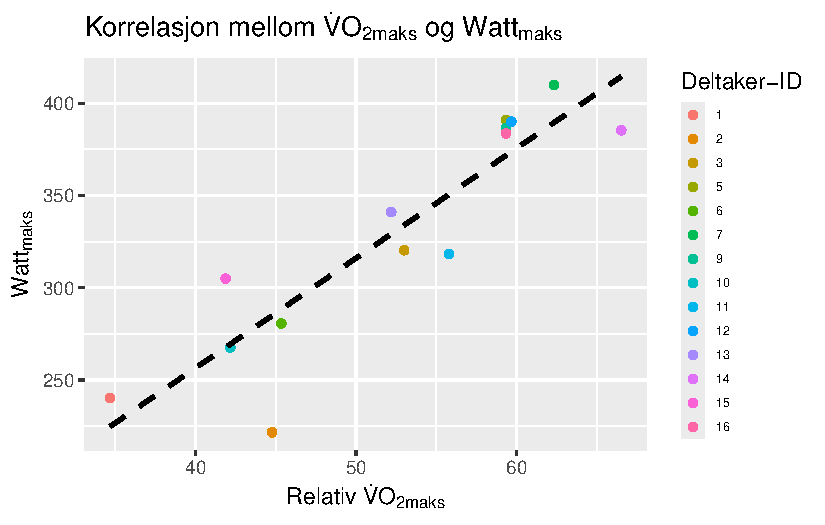
\includegraphics{01-reliabilitet_files/figure-pdf/unnamed-chunk-10-1.pdf}

}

\caption{Figur 1: Hvert punkt = én observasjon}

\end{figure}%

\paragraph{Diskusjon}\label{diskusjon}

Basert på de observerte resultatene fra testing av \(\dot{V}O_{2maks}\),
kan det konkluderes med at metoden vi har anvendt har høy reliabilitet.
Resultatene indikerer at vi måler det ønskede på en pålitelig måte, med
minimal variasjon i måleutstyret mellom testene.

Dette gir oss en trygghet i at vi med relativt stor sikkerhet kan
evaluere effekten av et treningsprogram ved å gjennomføre gjentatte
tester før og etter treningsperioder.

\bookmarksetup{startatroot}

\chapter{Assignment 2: Regression models, predicting from
data}\label{assignment-2-regression-models-predicting-from-data}

\section{Introduksjon}\label{introduksjon-1}

En regresjonsmodell er en modell som kvantifiserer forholdet mellom en
eller flere uavhengige variabler og en avhengig variabel. Innen medisin
er regresjon den analysemtoden som er hyppigst anvendt. Det finnes
forskjellige regresjonsmodeller. De vanligste er lineær regresjon,
polynominal regresjon og logistisk regresjon. Hva man har av datasett
vil bestemme hvilken regresjonsmodell som egner seg best å benytte
(Pisică et al. 2022).

En lineær regresjonsmodell er en modell der en kan estimere verdien av
en avhengig variabel basert på verdien av andre kjente uavhengige
variabler (Pisică et al. 2022). I en slik modell benyttes en rett linje
for å lage en modell som beskriver dataen. Følgende funksjon benyttes
for å skape det lineære plottet:

y\textsubscript{i} = b\textsubscript{0} +
b\textsubscript{1}x\textsubscript{i} + e\textsubscript{i}

der y\textsubscript{i} er den avhengige variabelen som kan estimeres ved
å benytte de uavhengige variablene b\textsubscript{1}x\textsubscript{i}
og b\textsubscript{0}. b\textsubscript{0} er skjæringspunktet til grafen
og b\textsubscript{1} er stigningstallet til grafen.

\section{Part 1 - Lactate thresholds}\label{part-1---lactate-thresholds}

\subsection{Metode}\label{metode-2}

Dataene ble organisert i et mer hensiktsmessig format (tidy data) for å
forenkle videre analyse og modellering. Deretter ble ulike
regresjonsmodeller anvendt for å representere dataene. Nye
skjæringspunkter ble tegnet opp for å illustrere treningsintensitet ved
forskjellige laktatnivåer.

\subsection{Resultat}\label{resultat-1}

\begin{figure}

\centering{

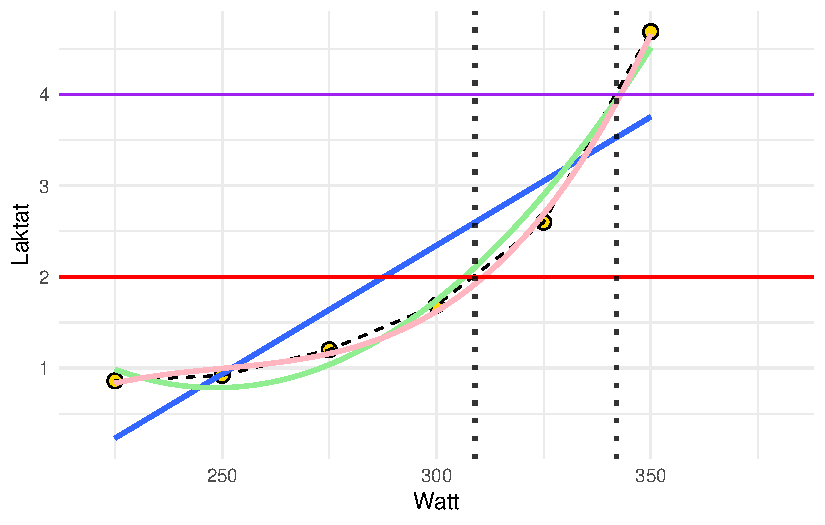
\includegraphics{02-regression-models_files/figure-pdf/fig-fig1-1.pdf}

}

\caption{\label{fig-fig1}Figur 1: Gule punkter = laktat og watt, blå
linje = lineær regresjon, grønn linje = andregradsligning, rosa =
tredjegradsligning.}

\end{figure}%

\subsection{Diskusjon}\label{diskusjon-1}

Vi har valgt å se på subject 10 fra datasettet Cyclingstudy. Vi gjør om
datasettet til tidydata. Dette gjør vi for å gi watt og laktat hver sine
verdier. Vi plotter inn laktatverdier og wattverdier (gule punkter).
Deretter tegner vi en stiplet linje som følger punktene. Vi gjør en
regresjonsanalyse, først en lineær modell (blå linje), deretter en
andregradsligning (grønn) og til slutt en tredjegradsligning (rosa).
Disse bruker vi for å observere hvilken modell som passer best i dette
tilfellet.

For å understreke hvor unøyaktig den lineære modellen er i dette
tilfellet, kan man på øyemål se at laktaten på 300W viser omtrent 2.4
mmol \textbf{×} L-1. Den faktiske laktaten på 300W er 1.69 mmol
\textbf{×} L-1 Figure~\ref{fig-fig1}.

\section{Part 2 - Predicting sizes of DNA
fragments}\label{part-2---predicting-sizes-of-dna-fragments}

\subsection{Metode}\label{metode-3}

For å predikere kalibreringskurven til qPCR, må en rekke prosesser på
molekylærlaboratoriet gjennomføres før dataene kan analyseres i R
Studio.

For å utføre en PCR på en 2\% agarosegel, ble det først tatt helblod fra
en forsøksperson for å ekstrahere DNA. Helblodet gjennomgikk ulike
prosesser hvor forskjellige løsninger og primere ble tilsatt. Dette
resulterte i et PCR-produkt. En elektroforese ble deretter kjørt for å
separere DNA-fragmentene fra PCR-reaksjonen. Etter fullført
elektroforese ble det tatt et bilde av 2\% agarosegelen.

Bildet fra elektroforesen ble analysert ved hjelp av ImageJ/Fiji, og
videre dataanalyser ble utført i R og R Studio. PCR-reaksjoners
effektivitet bestemmes av primerdesign og deres spesifisitet.

\subsection{Resultat}\label{resultat-2}

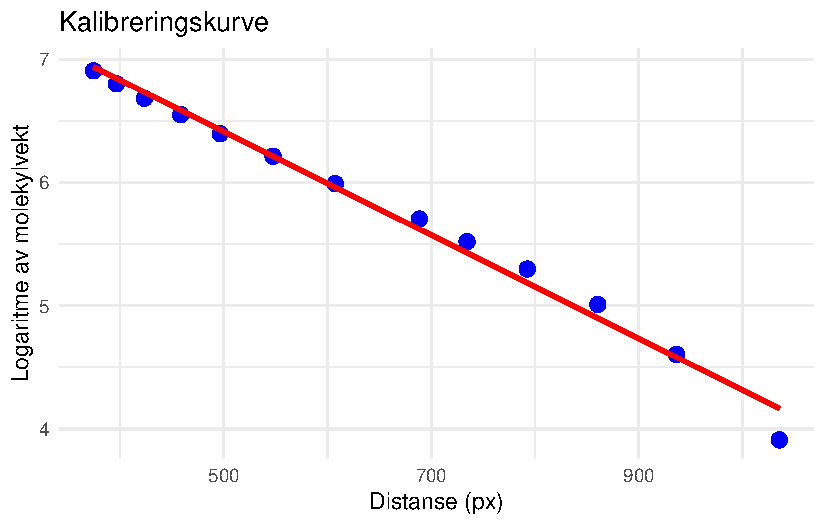
\includegraphics{02-regression-models_files/figure-pdf/unnamed-chunk-3-1.pdf}

\begingroup\fontsize{10}{12}\selectfont

\begin{longtable}[t]{>{}c>{}c>{}c}
\caption{Predikerte molekylvekter for ukjente distanser}\\
\toprule
\cellcolor[HTML]{404080}{\textcolor{white}{\textbf{Båndnummer}}} & \cellcolor[HTML]{404080}{\textcolor{white}{\textbf{Distanse (px)}}} & \cellcolor[HTML]{404080}{\textcolor{white}{\textbf{Predikert molekylvekt (bp)}}}\\
\midrule
\textbf{\cellcolor{gray!10}{1}} & \cellcolor[HTML]{F0F0FF}{\cellcolor{gray!10}{1208.5}} & \cellcolor[HTML]{F0F0FF}{\cellcolor{gray!10}{\cellcolor{red!25}31.22}}\\
\textbf{2} & \cellcolor[HTML]{F0F0FF}{600.5} & \cellcolor[HTML]{F0F0FF}{\cellcolor{yellow!25}400.05}\\
\textbf{\cellcolor{gray!10}{3}} & \cellcolor[HTML]{F0F0FF}{\cellcolor{gray!10}{18.5}} & \cellcolor[HTML]{F0F0FF}{\cellcolor{gray!10}{\cellcolor{green!25}4595.75}}\\
\textbf{4} & \cellcolor[HTML]{F0F0FF}{383.5} & \cellcolor[HTML]{F0F0FF}{\cellcolor{green!25}994.09}\\
\textbf{\cellcolor{gray!10}{5}} & \cellcolor[HTML]{F0F0FF}{\cellcolor{gray!10}{408.5}} & \cellcolor[HTML]{F0F0FF}{\cellcolor{gray!10}{\cellcolor{green!25}895.12}}\\
\addlinespace
\textbf{6} & \cellcolor[HTML]{F0F0FF}{436.5} & \cellcolor[HTML]{F0F0FF}{\cellcolor{green!25}795.93}\\
\textbf{\cellcolor{gray!10}{7}} & \cellcolor[HTML]{F0F0FF}{\cellcolor{gray!10}{470.5}} & \cellcolor[HTML]{F0F0FF}{\cellcolor{gray!10}{\cellcolor{green!25}690.14}}\\
\textbf{8} & \cellcolor[HTML]{F0F0FF}{508.5} & \cellcolor[HTML]{F0F0FF}{\cellcolor{green!25}588.45}\\
\textbf{\cellcolor{gray!10}{9}} & \cellcolor[HTML]{F0F0FF}{\cellcolor{gray!10}{559.5}} & \cellcolor[HTML]{F0F0FF}{\cellcolor{gray!10}{\cellcolor{yellow!25}475.12}}\\
\textbf{10} & \cellcolor[HTML]{F0F0FF}{618.5} & \cellcolor[HTML]{F0F0FF}{\cellcolor{yellow!25}370.95}\\
\addlinespace
\textbf{\cellcolor{gray!10}{11}} & \cellcolor[HTML]{F0F0FF}{\cellcolor{gray!10}{696.5}} & \cellcolor[HTML]{F0F0FF}{\cellcolor{gray!10}{\cellcolor{yellow!25}267.44}}\\
\textbf{12} & \cellcolor[HTML]{F0F0FF}{742.5} & \cellcolor[HTML]{F0F0FF}{\cellcolor{yellow!25}220.51}\\
\textbf{\cellcolor{gray!10}{13}} & \cellcolor[HTML]{F0F0FF}{\cellcolor{gray!10}{798.5}} & \cellcolor[HTML]{F0F0FF}{\cellcolor{gray!10}{\cellcolor{yellow!25}174.34}}\\
\textbf{14} & \cellcolor[HTML]{F0F0FF}{862.5} & \cellcolor[HTML]{F0F0FF}{\cellcolor{yellow!25}133.3}\\
\textbf{\cellcolor{gray!10}{15}} & \cellcolor[HTML]{F0F0FF}{\cellcolor{gray!10}{935.5}} & \cellcolor[HTML]{F0F0FF}{\cellcolor{gray!10}{\cellcolor{red!25}98.14}}\\
\addlinespace
\textbf{16} & \cellcolor[HTML]{F0F0FF}{993.5} & \cellcolor[HTML]{F0F0FF}{\cellcolor{red!25}76.94}\\
\bottomrule
\end{longtable}
\endgroup{}

\section{Part 3 - Interpreting a regression
table}\label{part-3---interpreting-a-regression-table}

\subsection{Metode}\label{metode-4}

\subsection{Resultat}\label{resultat-3}

\begin{figure}[H]

{\centering 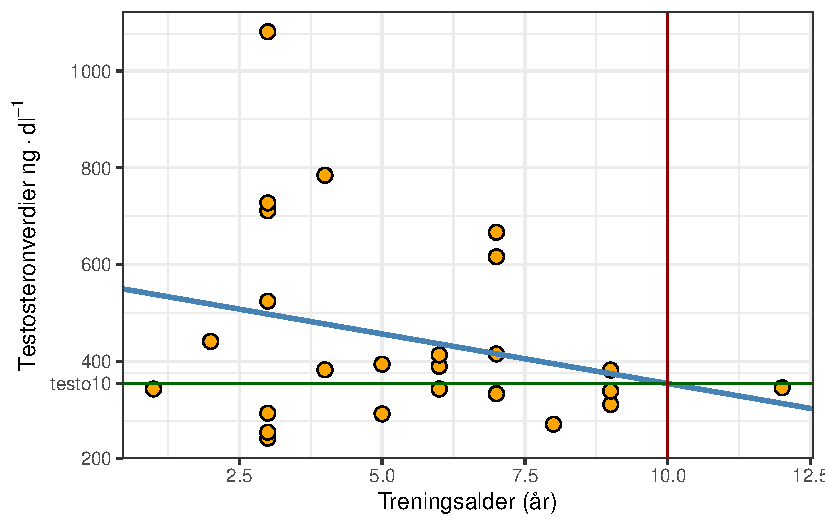
\includegraphics{02-regression-models_files/figure-pdf/tolkning av regresjonsmodell-1.pdf}

}

\caption{Figur 3: Sammenheng mellom treningsalder og testosteronverdier
i blodet}

\end{figure}%

\subsection{Diskusjon}\label{diskusjon-2}

Fra datasettet hypertrophy valgte vi å se på sammenhengen mellom
testosteronkonsentrasjon i blodet (ng \textbf{×} dl-1) og treningsalder
(antall år med trening). Den lineære modellen forteller at
testosteronkonsentrasjonen i blodet synker med 20.51 ng \textbf{×} dl-1
for hvert treningsår. Etter 10 år med trening, estimerer den lineære
modellen et testosteronnivå på 354.26 ng \textbf{×} dl-1.

Analysen av dataene viser en p-verdi på 0,1779, noe som indikerer at det
ikke er statistisk signifikant bevis for en sammenheng mellom
treningsalder og nivået av testosteron i blodet. Siden p-verdien er
høyere enn det vanlige signifikansnivået på 0,05, kan vi ikke avvise
nullhypotesen, som antyder at det ikke er noen betydelig effekt eller
sammenheng mellom de to variablene i dette datasettet. Dette betyr at
variasjonen i testosteronnivåer ikke ser ut til å være relatert til hvor
lenge individene har trent.

I analysen av sammenhengen mellom treningsalder og testosteronnivåer i
blodet ses det en t-verdi på 6.250. Den høye t-verdien på 6.250, og en
p-verdi på 0,1779. Denne p-verdien er høyere enn det vanlige
signifikansnivået på 0,05, noe som betyr at vi ikke har tilstrekkelig
statistisk bevis for å avvise nullhypotesen. Selv om t-verdien indikerer
en mulig sammenheng mellom treningsalder og testosteronnivå, er det ikke
nok evidens til å konkludere med at denne sammenhengen er signifikant.
Dermed kan vi konkludere med at selv om det kan være en tendens til en
sammenheng mellom treningsalder og testosteronnivåer, er resultatene fra
denne analysen ikke sterke nok til å si at treningsalder har en reell
effekt på testosteronnivåene i blodet.

\bookmarksetup{startatroot}

\chapter{Assignment 3: Drawing inference from statistical models, and
statistical
power}\label{assignment-3-drawing-inference-from-statistical-models-and-statistical-power}

\section{Oppgave 1}\label{oppgave-1}

Ved bruk av regresjonsmodellen lm1 og lm2 skal jeg i denne oppgaven
definere begrepene estimat, SE (standardfeil), T-verdi og P-verdi ut
ifra det vi vet fra prosessen med og gjennomføre en studie med et
tilfeldig utvalg.

Estimat: Representerer gjennomsnittet av det vi har målt i utvalget. Så
i vårt tilfelle viser estimatet gjennomsnitt på den ene variabelen (y) i
de to forskjellige utvalgene.

SE (standardfeil): SE defineres som hvor mye vi kan forvente at
gjennomsnittet kan variere hvis du hadde valgt en annen tilfeldig gruppe
fra populasjonen. I tillet vi har er det ett SE på 3,539 som vil si hvis
vi gjennomfører en ny studie med ett annet utvalg, vil vi kunne forvente
en endring i gjennomsnitttet på 3,539. Jo lavere SE vi har, jo mer
sikker er vi på at utvalget representer populasjonen bedre.

T-verdi: En t-verdi er et statistisk mål som anvendes i t-tester for å
vurdere om forskjellen mellom to grupper, eller mellom et
prøvegennomsnitt og en kjent verdi, er signifikant. Den uttrykker hvor
stor den observerte forskjellen er i forhold til den forventede
variasjonen i dataene, representert ved standardfeilen. En høy t-verdi
indikerer at forskjellen er betydelig i forhold til variasjonen, noe som
kan tyde på en reell effekt. T-verdien i m1: 1,47, T-verdi m2: 3,276

P-verdi: En p-verdi er et statistisk mål som uttrykker sannsynligheten
for å få et resultat som er minst like ekstremt som det observerte, gitt
at nullhypotesen er sann. Den brukes til å vurdere om en observert
effekt eller forskjell kan forklares med tilfeldigheter. En lav p-verdi
(for eksempel mindre enn 0,05) antyder at resultatet er lite sannsynlig
å ha oppstått ved tilfeldigheter alene, og nullhypotesen kan derfor
avvises. P-verdien gir altså en indikasjon på hvor sterk evidensen er
mot nullhypotesen, men sier ikke noe om effektenes størrelse eller
praktiske betydning.

\section{Oppgave 2}\label{oppgave-2}

Forskjellene i de to studiene (m1 og m2) er prøvestørrelsen. M2 har n=8
mens m2 har n=40. Studien med større prøvestørrelse vil gi mer
pålitelige svar, da den statestistiske styrken er høyere, og
sansynligheten for at det faktisk er funnet en sann effekt er større.
Dette fordi med færre prøvestørrelser er man mer sårbar for tilfeldige
svar, og dermed usanne sanheter.

\section{Oppgave 3}\label{oppgave-3}

Vi bruker skyggelagte områder i de ekstreme tilfellene ved nedre og øvre
del for og utelukke uteliggere, det vil si de ekstreme tilfellene som
ikke er representative for gjennomsnittet i prøvegruppen.

\section{Oppgave 4}\label{oppgave-4}

Standardfeilen (SE) er et estimat på hvor mye feilene skal variere fra
prøve til prøve, standardavviket er det faktiske variasjonen. Jo flere
prøvepersonen det er, jo likere vil SE og standardavviket være, fordi SE
forutsier dette.

\section{Oppgave 5}\label{oppgave-5}

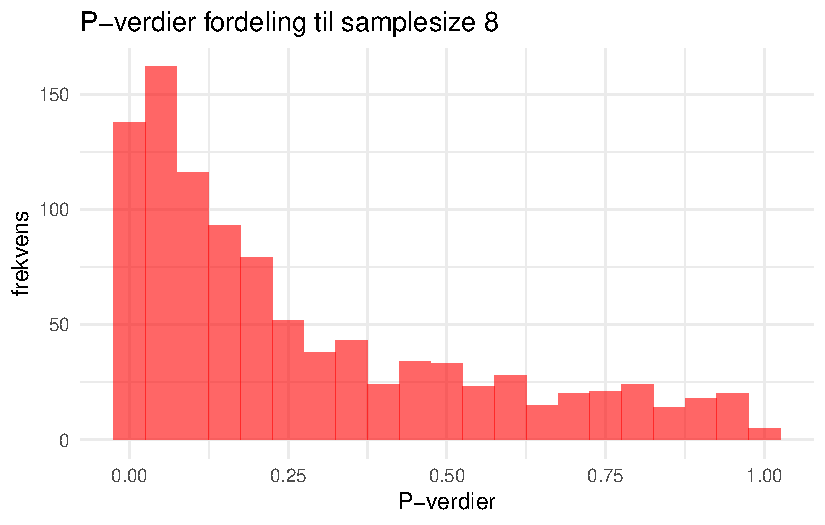
\includegraphics{03-statistical-inference_files/figure-pdf/P-verdi histogram SS8-1.pdf}

Histogrammet for modellen med utvalgsstørrelse på 8 viser en tydelig
overvekt av høye p-verdier. Dette reflekterer den lave statistiske
styrken som oppstår når man utfører studier med en så liten
utvalgsstørrelse.

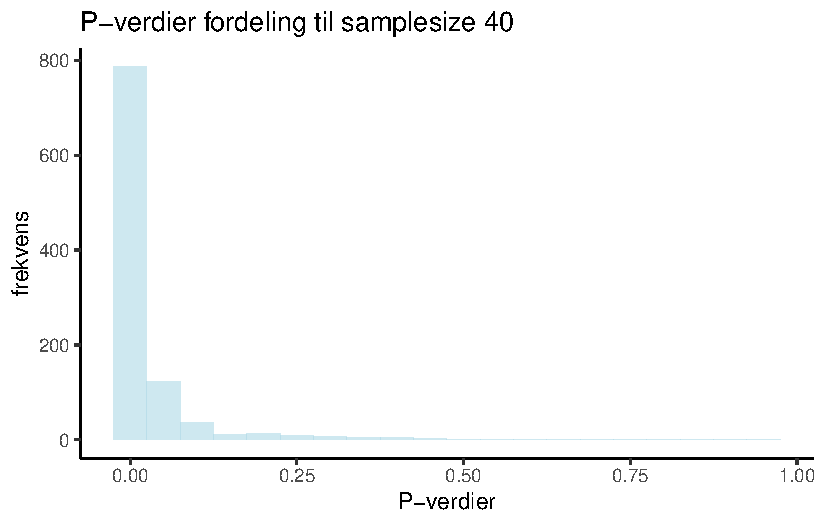
\includegraphics{03-statistical-inference_files/figure-pdf/P-verdi histogram SS40-1.pdf}

I histogrammet for modellen med utvalgsstørrelse på 40 ser vi at flere
observasjoner er konsentrert rundt lavere p-verdier. Dette skyldes at en
større utvalgsstørrelse gir høyere statistisk styrke.

\section{Oppgave 6}\label{oppgave-6}

For studiene med utvalgsstørrelse på 8 er det 227 som viser statistisk
signifikans, mens for studiene med utvalgsstørrelse på 40 er antallet
hele 865. Dette illustrerer tydelig hvor stor betydning
utvalgsstørrelsen har for resultatene i analysene. I dette tilfellet er
terskelen for signifikans (p-verdi) satt til 0.05

\section{Oppgave 7}\label{oppgave-7}

Konklusjonen på disse studiene viser til at jo større utvalg det er, jo
høyere statestisisk styrke. (power). Med høyere statestistisk styrke jo
mer sansynlig er det at vi har funnet en sanhet, og ikke falsk sannhet
som i tilfellet hvis det er lav statestistisk styrke, som i tilfellet
med n=8 (færre forsøkspersoner)

\section{Oppgave 8}\label{oppgave-8}

Ved å gjennomføre 1000 gjentatte studier med et signifikansnivå satt til
0,05, kan vi forvente rundt 50 falske positive resultater. I mine
beregninger fant jeg at det var r \texttt{false\_positive\_8} falske
positive for studiene med en utvalgsstørrelse på 8, og r
\texttt{false\_positive\_40} for studiene med en utvalgsstørrelse på 40.
Hvis signifikansnivået senkes til 0,025, reduseres antall falske
positive noe. Da vil studiene med en utvalgsstørrelse på 8 gi r
\texttt{false\_positive\_8\_alpha0.025} falske positive, mens studiene
med 40 deltakere gir r \texttt{false\_positive\_40\_alpha0.025} falske
positive.

\bookmarksetup{startatroot}

\chapter{Studiedesign}\label{studiedesign}

I denne oppgaven skal jeg velge meg ut fem forskjellige studier og se på
hvordan disse er gjennomført i sin helhet, ved styrker og svakheter i
prosjektene. Studiene jeg har valgt og se på er studier som vurderer
hvordan blokklegging av HIT-trening (Høy-intensitets trening) påvirker
utholdenhetsprestasjonen til godt trente utholdenhetsutøvere. De ønsker
og finne en måte og optimalisere den intensive treningen for og få mest
mulig effekt ved og organisere det på en annen måte enn tidligere. I
studiene sammenligner de ofte da perioder med fler HIT øker på en
kortere periode istedenfor tradisjonell måte der HIT øktene er mer
fordelt utover en gitt periode.

Det har i nyere tid blitt mer og mer populært og se etter måter og
optimalisere trening, spesielt for godt trente utøvere. Vi ser at for
godt trente utøvere kreves det ekstra stimuli for at det skal skje
endring, og ut ifra dette har blokk periodisering blitt populært. Dette
er en måte og prioritere visse egenskaper over en viss tid samtidig som
du vedlikeholder andre egenskaper. Du setter kroppen i en større
utfordring, og med det store stimuliet krever du at kroppen gjør en
endring og tilpasser seg (Issurin 2008).

Bent Rønnestad er en forsker som har sett mye på dette med
blokkperiodisering av HIT-økter sammenlignet med tradisjonell oppbygning
av HIT-økter. I studien til Rønnestad med overskriften
«Blokkperiodisering av høyintensive intervaller gir bedre
treningseffekter hos trente syklister» (B. R. Rønnestad and Mujika 2014)
gjør de en studie som ser på forskjellene i effekten på to metoder for
organisering av utholdenhetstrening. Den ene gruppen (forsøksgruppa)
kjører første uken med fem HIT-økter, etterfulgt av tre uker med en
HIT-økt per uke og hovedfokus på lavintensitetstrening. Kontrollgruppen
fortsetter å kjøre tradisjonelt oppsett av periodiseringen, der de
gjennomfører fire uker med to HIT-økter per uke kombinert med
lavintensiv trening. De ser på faktorene som VO2max, Wmax (topp
kraftutgang) og melkesyreterskel, sammenlignet med TRAD, hos trente
syklisterVO2max, Wmax (topp kraftutgang) og melkesyreterskel,
sammenlignet med kontrollgruppen, hos trente syklister. Hypotesen i
artikkelen er at blokkperiodisering vil gi bedre tilpasninger enn
tradisjonell periodisering hos trente syklister. Det samme gjelder
hypotesen i studien (Bent R. Rønnestad et al. 2022), som så på effekten
av 6-dagers HIT-blokk på utholdenhetsprestasjonene til langrennsløpere,
mål ved endringer i VO2max, maksimalt oksygenopptak, kraftutgang, og
muskelkapillaritet. I likhet med den andre studien var hypotesen at
gruppen som gjennomførte HIT trening i blokk ville forbedre sine
prestasjonsindikatorer sammenlignet med gruppen som gjennomførte
tradisjonell trening.

En annen studie fra (Almquist et al. 2022) er hypotesen at
blokkperiodisering av HIT-økter ville føre til større forbedringer i
utholdenhetsprestasjoner enn tradisjonell trening, men i denne studien
ble ikke hypotesen støttet da resultatene ikke stemte overens med dette.
Mens i de to siste studiene jeg skal se på, hhv. (Breil et al. 2010) og
(Solli, Tønnessen, and Sandbakk 2019) viser begge hypotesene til at de
tror blokkperiodisering av HIT-trening vil føre til bedre
utholdenhetsprestasjoner. Kort oppsummert kan vi se at de fleste
studiene rammer inn forskingsproblemet som hypoteser, mens studien
(Almquist et al. 2022) formulerer det som et utforskende spørsmål. Vi
kan si at hypotesedrevet forskning passer godt når vi har lyst til og
teste det spesifikke, målbare antakelser, mens mer spørsmål kan være
bedre når forskninger er i en tidlig fase ved at det kan forskes
bredere. En årsak til logikken bak hypotesene er at bolkgruppene vil få
en større mekanisk belastning over en kortere tidsperiode som er et
sentralt signal til tilpasning.

Når det gjelder studiedesignet har studiene (Bent R. Rønnestad et al.
2022), (B. R. Rønnestad and Mujika 2014), (Breil et al. 2010) et
randomisert kontrollert design. Randomiserte studier vil si at
forsøkspersonene i gruppen er tilfeldig plassert i enten kontroll, eller
blokktrenings-gruppen. Deltakere bør kvalifisere seg og gi samtykke for
randomisering (Hulley et al. 2013). Det at studiene er randomiserte
styrker studien ved at de utelukker påvirkningen av andre faktorer. Det
minsker sjansen for skjevhet og gjør resultatene mer pålitelige.
(Almquist et al. 2022) er ikke fullstendig randomisert kontrollert
design da gruppene er uten strengt randomisert fordeling, dette kan være
en svakhet ved studien. (Solli, Tønnessen, and Sandbakk 2019) skiller
seg litt ut fra de andre studiene ved at den undersøker en enkelt
forsøksperson.

Når det gjelder utvalget i de forskjellige studiene ligger dette på
rundt 20 forsøkspersoner, der de fordeler 50/50 mellom kontroll gruppe
og intervensjonsgruppe. Studien til (Solli, Tønnessen, and Sandbakk
2019) er spesiell da det er en enkelmansstudie, og vi kan da si at den
ikke representerer ett tilfeldig utvalg av populasjonen og gir derfor
ikke et bilde på hele befolkningen, og resultatene kan være tilfeldige.
I de resterende studiene kan vi si at det hadde vært fordelaktig og hatt
ett større utvalg for og kunne si noe mer om det generelle i
befolkningen. Ved færre forsøkspersoner kan det være større
sannsynlighet for at resultatene har kommet ved en tilfeldighet. I alle
studiene er det også plukket utøvere som er godt trente og på ett høyt
nivå fra før, noe som vil si at resultatene kan sies og være relevante
for denne gruppen personer, men ikke nødvendigvis for gjennomsnitt
personen i populasjonen. I alle studiene måtte du være kvalifisert for
og kunne være med, gjennom og ha visse resultater, dermed var det ikke
et helt tilfeldig utvalg.

Hvis vi ser på hvordan gjennomføringen var i studiene, brukte alle
studiene pre- og post tester for å måle endringer i
utholdenhetskapasitet, VO2max og andre fysiologiske parametere. I
studiene (Bent R. Rønnestad et al. 2022), (B. R. Rønnestad and Mujika
2014) og (Almquist et al. 2022) ble det gjennomført tester som testen
både fysiologiske verdier og prestasjonsmål, prestasjonsmål er for
eksempel en 20min/40min alt ut test der du ser om prestasjonen har blitt
bedre. Det er en styrke og både se på fysiologiske faktorer og
prestasjon, da vi kan få ett større bilde om det faktisk har ført til
endringer. I (Solli, Tønnessen, and Sandbakk 2019) ble resultater i
konkurranser brukt, dette er ett prestasjonsmål, men det er vanskelig og
si om det er andre faktorer som skaper støy i forskingen og om vi
faktisk klarer og finne ut hva som førte til endringer i resultater.

De fleste studiene brukte t-tester og gjentatte målinger ANOVA for og se
forskjeller i resultatene pre- og post intervensjonen. Ved bruk av dette
kan man gjøre det mulig og se endinger i variabler er statistisk
signifikante, og dermed støtter eller avkrefter hypotesene. Fire av
studiene brukte også grafer og deskriptiv statistikk for å vise at
treningsbelastningen mellom gruppene og utgangspunktet til
forsøkspersonene var likt, med unntak av (Solli, Tønnessen, and Sandbakk
2019) som ikke hadde kontrollgruppe og derfor ikke noe om å sammenligne
med.

Når det gjelder resultater så konkluderte (Breil et al. 2010)med at
HIT-gruppen forbedret VO2max med 6\%, og relativ topp kraftutgang med
5,5\% sammenlignet med kontrollgruppen. Det var ingen signifikant ending
i alt ut test for noen av gruppene. I dette tilfellet støttet
resultatene hypotesen ved at en intensiv HIT-bolk vil gi større
forbedringer på VO2max og kraftutgang enn tradisjonell trening. (B. R.
Rønnestad and Mujika 2014), (Bent R. Rønnestad et al. 2022) viste begge
studiene at gruppen som gjennomførte HIT-blokk trening hadde størst
forbedringer på fysiologiske og prestasjonsmål. I begge tilfellene hadde
Rønnestad støttet hypotesen. (Almquist et al. 2022) støttet ikke
hypotesen ved at han ikke fant noe signifikante forskjeller mellom
gruppene på sykkelprestasjon.

\bookmarksetup{startatroot}

\chapter{Assignment 5: Analyzing repeated measures
experiments}\label{assignment-5-analyzing-repeated-measures-experiments}

\section{Introduksjon:}\label{introduksjon-2}

Styrketrening er en viktig del av fysisk trening. Styrketrening er
viktig i ett helseperspektiv ved å forebygge helsemessige utfordringer,
dette kan for eksempel være muskelatrofi og svekket beinstyrke
(Jespersen, Pedersen, and Beyer 2003). Styrketrening har også vist seg
og være viktig for og forbedre fysisk prestasjon (B. R. Rønnestad and
Mujika 2014). Maksimal styrketrening avhenger hovedsakelig av
muskelmasse, og det er en rekke faktorer man kan påvirke for og øke
muskelmasse og muskelstyrke. (Raastad et al. 2010). Hvordan fordele
treningsvolum, frekvens og motstand optimalt kan variere fra person til
person, her spiller genetikken også inn. Treningsvolum i
styrkesammenheng vil si antall sett per muskelgruppe i løpet av en uke.
(Grgic et al. 2022). Fokuset rundt treningsvolum og styrketrening har i
lengre tid vært ett stort tema. Det er vist i tidligere studier at ett
lavt treningsvolum har ført til samme forbedringer som moderat
treningsvolum. (Mitchell et al. 2012). Det kan spekuleres om det også er
forskjeller når det gjelder godt styrketrente personer og dårlig
styrketrente personer. Der det kan tyde på at det vil kreves ett større
stimuli jo høyere nivå du er på. (Hughes, Ellefsen, and Baar 2018).

Selv om vi de aller fleste vet at styrketrening er viktig for helsa, er
det mange personer som ikke gjennomfører regelmessig styrketrening.
Begrensinger kan være kunnskap og evnen til og klare og sette av tid og
prioritere det. trene (Choi et al. 2017). Derfor kan det være veldig
hensiktsmessig og kunne finne ut mer rundt hvor mye stimuli og
treningsvolum som faktisk kreves for og klare og få de adaptasjonene vi
vil og de positive helsemessige gevinstene. Vi ser også at veldig mange
i samfunnet nå blir mer og mer stillesittende, kan dette skape store
problemer for helsa til mange personer i samfunnet. Studier viser også
at muskelmasse og muskelstyrke reduseres spesielt ved økende alder, og
rundt 50 år spesielt. Ved redusert styrke kan det føre til en rekke
negative konsekvenser. Det at man som eldre mister muskelmasse er en
naturlig prosess, men ved gjennomføring av styrketrening kan vi bremse
denne utviklingen. (Marzetti and Leeuwenburgh 2006).

Studiene (Rhea et al. 2002) viste at gruppen som trente tre sett per
øvelse hadde en større økning i muskelstyrke sammenlignet med den
gruppen som trente med bare ett sett. (Bent R. Rønnestad et al. 2007)
fant også ut at tre sett hadde bedre resultater enn gruppen som trente
ett sett. Basert på studier som er gjort tidligere har denne studien som
mål og se på forskjeller i muskelstyrke og muskelmasse der en gruppe
trener med ett sett og en annen gruppe kjører tre sett. Det gjennomføres
på beina. Resultatene kan finne ut hvordan forskjellige treningsvolumer
påvirker styrken vår og muskelmassen.

\section{Metode}\label{metode-5}

\#Deltagere

I studien ble det rekruttert 41 mannlige og kvinnelige deltagere. Det
var noen krav som måtte dekkes for og kunne være med i studien, og det
var at personene måtte være mellom 18-40 år og ikke røyke. Personene
kunne ikke ha trent mer enn en ukentlig styrkeøkt det siste året,
samtidig som de ikke skulle ha noe nedsatt muskelstyrke ved noen
tidligere skader eller lignende. De skulle heller ikke gå på noe
medisiner som kunne påvirke eller forstyrre effektene for treningen.
Etter studien ble sju personer tatt vekk fra dataanalysen fordi de ikke
hadde gjennomført tilstrekkelig av de obligatoriske øktene (85\%) i
treningsintervensjonen.

\begingroup
\fontsize{12.0pt}{14.4pt}\selectfont
\setlength{\LTpost}{0mm}

\begin{longtable}{lrrr}

\caption{\label{tbl-kar}Karakteristikk av deltakerene}

\tabularnewline

\toprule
Variable & N & Avg & SD \\ 
\midrule\addlinespace[2.5pt]
age & 34 & 22.8 & (3) \\ 
height & 34 & 174.8 & (10) \\ 
weight & 34 & 69.7 & (11.9) \\ 
\bottomrule

\end{longtable}

\begin{minipage}{\linewidth}
Avg = Gjennomsnitt, SD = Standardavvik\\
\end{minipage}
\endgroup

\section{Intervensjon:}\label{intervensjon}

Perioden ble gjennomført i løpet av 12-ukers styrketrening av hele
kroppen. Underekstremitetene ble trent unilateralt. Dette gjør det mulig
å gjennomføre forskjellig treningsvolum på beina. Det ble gjennomført
lavt volum på det ene beinet og moderat på det andre. Det ble
gjennomført ett sett på beinet som hadde lavt treningsvolum, og tre sett
på det med moderat treningsvolum. Det ble gjennomført treningsøkter to
til tre ganger i uken. Før hver treningsøkt gjennomførte personene en
standardisert oppvarmingsprotokol. Den bestod av 5 minutter sykling på
ergometersykkel, deretter ti repetisjoner av kroppsvektøvelser som
push-ups, sit-ups, rygg hev og knebøy. Etter dette gjennomførte de ett
sett med ti repetisjoner på 50\% av 1RM (maksimalt løft) for hver
styrkeøvelse. De tre beinøvelsene som ble gjennomført var unilateralt
beinpress, leg-curl og kneekstensjon. Under teningsøkene hadde personene
90 til 180 sekunder pause mellom hver sett. Når det gjelder kosthold ble
deltagerne bedt om å logge kosthold, samtidig som de fikk et
standardisert energipåfyll, hhv. 0,16 g protein, 11,2 g karbohydrater og
0,5 g fett per kilo kroppsvekt. Dette var for og sikre at deltagerne
fikk ett likt tilskudd av energi etter trening slik at ikke
restitusjonen ble påvirket forskjellig på grunn av dette.

\section{Målinger}\label{muxe5linger}

I studien ble det brukt en repetisjon maksimum (1RM) i kneekstensjon som
mål på maksimal styrke. Det ble gjennomført en standardisert oppvarming
i forkant av mål på maksimal styrke. Denne oppvarmingen bestod av 10, 6
og 3 repetisjoner på en belastning tilsvarende 50, 75 og 85 \% av antatt
1RM. Videre gjennomførte deltakeren fire til seks forsøk der de økte
belastning per sett og til slutt til den belastninger der de ikke klart
og løfte vekten. Den siste repetisjonen med fullt bevegelsesutslag ble
da definert som 1RM.

Det ble også målt andel fettfri masse før og etter intervensjons
perioden. Det ble mål ved bruk av dual-energy X-ray absorptiometry
(DXA), (Lunar Prodigy, GE Healthcare, Oslo, Norge). Det var
standardisert 48 timer opphold mellom siste styrkeøkt og DXA, samt at
deltakerne skulle faste 2 timer før test og avstå fra krevende fysisk
aktivitet de siste 48 timer.

\section{Dataanalyse og statistikk}\label{dataanalyse-og-statistikk}

De statiske analysene ble gjort i R studio. Det ble gjennomført enkle
lineære regresjonsmodeller for og se differansen mellom gruppene som
gjennomførte ett sett kontra tre sett. Det ble sett på mager muskelmasse
i beinet som trente ett sett kontra tre for og se endringer i
muskelmasse. Signifikansnivået i studien ble satt til p \textless{}
0,05. Dette vil da si at resultater som viser til en p-verdi under dette
blir ansett som statistisk signifikante.

\section{Resultater}\label{resultater}

Beinet som trente tre sett hadde en større økning i fettfri masse enn
beinet som trente ett sett. Forskjellen mellom gruppene oppgitt i gram
var r m1results. Figure~\ref{fig-1} viser hvor mange gram deltakerne
økte i fettfri masse fra pre- til posttest. I 1RM benpress var det en
gjennomsnittlig differanse oppgitt i kilo på r m2results.
Figure~\ref{fig-2} viser hvor mange kilo deltakerne økte i 1RM benpress
fra pre- til posttest.

\begin{figure}

\centering{

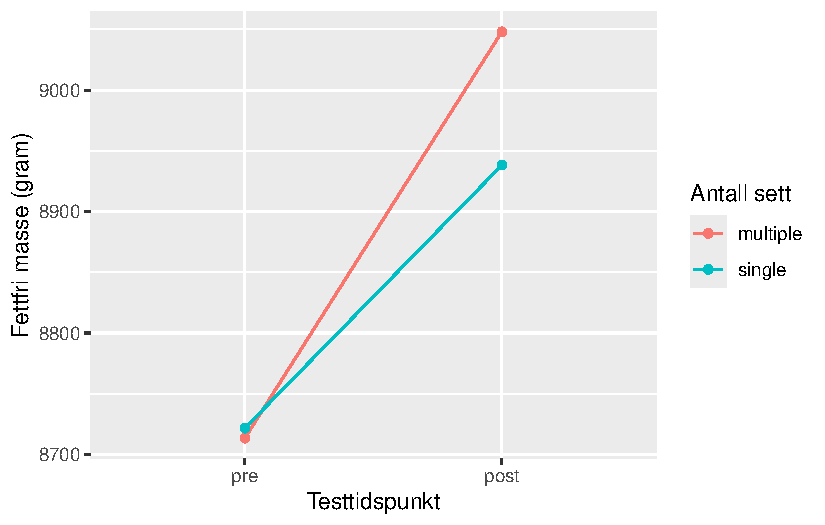
\includegraphics{05-repeated-measurements_files/figure-pdf/fig-1-1.pdf}

}

\caption{\label{fig-1}Gjennomsnittlig endring i fettfri masse mellom
pre- og posttest}

\end{figure}%

\begin{figure}

\centering{

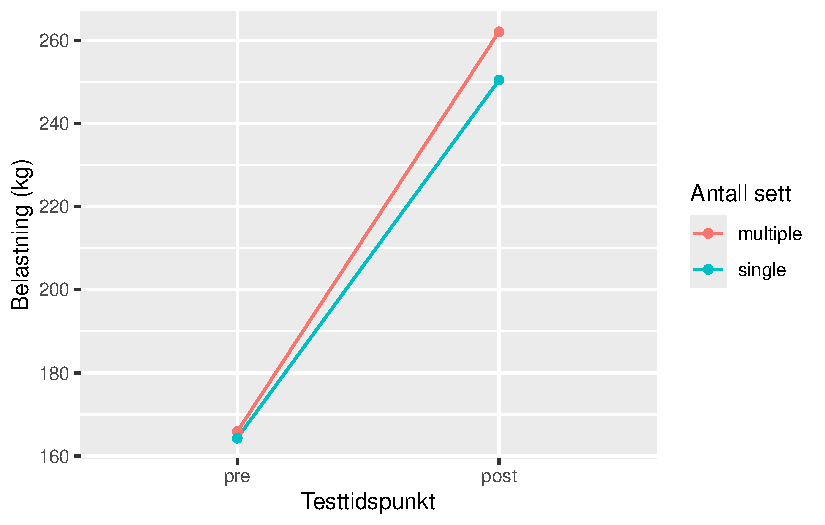
\includegraphics{05-repeated-measurements_files/figure-pdf/fig-2-1.pdf}

}

\caption{\label{fig-2}Gjennomsnittlig endring i benpress 1RM mellom pre-
og posttest}

\end{figure}%

\section{Diskusjon}\label{diskusjon-3}

Studien viste en tydelig forskjell i økningen av fettfri masse og 1RM
benpress mellom gruppene som trente ett sett og tre sett per øvelse.
Gruppens større fremgang med tre sett støtter teorien om et
dose-responsforhold, der et høyere treningsvolum fører til bedre
treningsadaptasjoner, som også er påvist av (Schoenfeld et al. 2017).

Det er likevel verdt å merke seg at deltakerne opplevde betydelig
fremgang i både styrke og fettfri masse i begge ben, uavhengig av
treningsvolum. Treningsprotokollen inkluderte to øvelser som belaster
forsiden av låret, med en frekvens på 2-3 økter per uke. Dette
resulterte i at det ukentlige volumet for beinet som trente ett sett per
øvelse lå på 4-6 sett totalt. I tråd med dette fant
(Androulakis-Korakakis, Fisher, and Steele 2020) at selv ett enkelt sett
med 6-12 repetisjoner, utført med høy innsats 2-3 ganger per uke, kan
føre til signifikante, men suboptimale, styrkeøkninger hos godt trente
individer. Disse funnene antyder at et lavt volum kan gi effektive
resultater, men et moderat volum gir mer optimale tilpasninger. For
personer med begrenset tid til styrketrening kan dette være nyttig
informasjon, da det viser at selv minimal innsats kan gi helsemessige og
fysiske fordeler, selv om økt volum gir bedre resultater.

\bookmarksetup{startatroot}

\chapter{Philosophy of science}\label{philosophy-of-science}

\section{Oppgave 1:}\label{oppgave-1-1}

I vitenskapen bruker vi vitenskapelige argumenter som en måte for og
rasjonelt og strukturelt måte kunne ha et bevis for og avkrefte eller
bekrefte en påstand. Vitenskapelige argumenter er grunnleggende for
vitenskapelige metode og den kritiske vurderingen av vitenskapelige
påstander. Vi kan skille mellom induktive og deduktive argumenter. I
deduktive argumenter er konklusjonen unngåelige dersom premissene er
sanne, og argumentet er da deduktivt gyldig hvis det oppfyller dette
kravet. Ett eksempel på et deduktivt argument kan være: Premiss 1: Alle
mennesker er dødelige. Premiss 2: Sokrates var ett menneske. Konklusjon:
Sokrates er dødelig. (Thurén 2022)

Induksjon er en type vitenskapelig argumentasjon som trekker generelle
konklusjoner ut fra spesifikke observasjoner, det vil si at vi trekker
konklusjoner om fremtiden basert på observasjoner fra fortiden. Vi
bruker denne måten og trekke konklusjoner på i både hverdagen og i
vitenskapen. For eksempel kan vi bruke eksempelet om solen. Premiss 1:
Sola har stått opp hver dag de siste 50 årene. Konklusjon: Solen vil stå
opp i morgen. (Vasserud 2024). Selv om det er lett og si at det er
logisk for oss at solen vil stå opp i morgen med det grunnlaget at den
alltid har stått opp, men det dukker opp vitenskapelige spørsmål rundt
dette. I det at vi konkluderer med at noe vil skje på grunn av at det
har skjedd før viser til at vi legger til grunn at fremtiden skal være
identisk med fortiden. Og kan vi da rettferdiggjøre induktive
slutninger? (Thurén 2022)

David Hume er en av de mest innflytelsesrike filosofene på 1700-tallet.
Hume hevdet at det var umulig og rasjonelt rettferdiggjøre bruken av
induksjon, og kom da opp med induksjonsproblemet. Humes problem med
induktiv argumentasjon gikk ut på at troen om at fremtiden vil følge de
samme mønstrene som i fortiden. Han sier at induksjon er en vanlig
tilnærming, men vi kan ikke bevise at fremtiden skal være lik fortiden,
noe som vil si at konklusjonen kan være sann, men det er ingen garanti.
Humes kritikk handler om det faktumet at induktiv argumentasjon
forutsetter ett skjult premiss, prinsippet om at fremtiden er lik
fortiden. Dette prinsippet kan da ikke bevises rasjonelt. Hvis vi prøver
å rettferdiggjøre dette ved bruk av induksjon havner vi i en
sirkulær-argumentasjon ved at vi bruker induksjon for og rettferdiggjøre
induksjon. Dette betyr at vi ikke rasjonelt kan bevise brukes av
induksjon uten forutsette det vi prøver og bevise. For og komme med
eksempler rundt dette bruker vi sola som tidligere i oppgaven. Vi sier
at solen kommer til og stå opp i fremtiden, basert på at den har stått
opp hver dag i fortiden. Selv om det er logisk og enkelt og si at sola
vil stå opp i morgen basert på at den har gjort det i alle år, er det
ingen garanti for at det skjer. Hume stiller spørsmålet: hvorfor skal vi
anta at morgendagen skal følge tidligere mønstre? (Holmen 2024)

En vanlig innvending mot Humes syn er at induksjon kan forsvares selv om
det ikke er noe garanti for at konklusjonen er sann. Det er såpass
fornuftig og tro at solen vil stå opp i morgen basert på at den alltid
har gjort det. Det er fornuftig å stole på induksjonen for og kunne
legge fremtidsplaner, selv om vi ikke kan garantere for fremtiden. Denne
innvendingen er basert på erfaringer mer enn rasjonalitet.
Vitenskapelige fremgang er i mange tilfeller basert på induksjon selv om
vi ikke kan bevise at disse slutningene er riktige. Det baseres da på at
det i flere tilfeller har stemt så godt at det er suksessen i praksis
som gjør at vi tror på det. Det blir ett eksempel på at det er sant helt
til det motsatte er bevist. Hume kan ha avvist denne innledningen ved og
si at det foresatt ikke er en rasjonell begrunnelse for induksjon. Selv
om induksjon er en praktisk måte og tenke på både i vitenskapen og i
hverdagen, er det ikke samme som logiske eller rasjonelle argumenter. Vi
vil hele veien ende opp med den samme sirkulær resonnementet som Hume
kritiserte. For Hume er poenget at uansett hvor lettvint og logisk det
er at fremtiden er lik fortiden, er det ingen garanti for og si dette.
(Holmen 2024)

Men for og kunne bringe verden fremover og i hverdagen vil det alltid
være induktive argumenter. Dette vil skape mindre bekymringer enn at vi
ikke kan planlegge morgendagen på bakgrunn av at vi ikke kan garantere
at sola står opp fremover.

\subsection{Oppgave 2}\label{oppgave-2-1}

Karl Popper var en av de mest innflytelsesrike vitenskapsfilosofiene,
han utviklet teorien om falsifikasjonisme som et svar på Humes problem
mot induksjon. Popper mente at problemet rundt induktiv argumentasjon
kunne forsvares ved fokus på forfalskningen fremover verifisering.
Popper mente at måle ved vitenskapen burde være å teste teorier ved og
motbevise dem, isteden for og prøve og bekrefte teorier ved bruk av
induksjon. Popper ville da utvikle falsifikasjonisme som ett svar på det
han mente var svakhetene rundt Humes argumenter rundt den induktive
argumentasjonen. Popper innså at det som Hume hadde påpekt var umulig å
verifisere en vitenskapelig teori basert på begrenset antall
observasjoner. (Tranøy 2024).\\
Popper ville heller at en god vitenskapelig teori måtte være
falsifiserbar. Noe som vil si at den må testes på en måte som beviser at
den er falsk. I eksempelet som er brukt i oppgaven med at sola vil stå
opp i morgen med premisset at den alltid har gjort det, er det hittil
umulig og bevise at det er falskt at det vil skje. Hvis en teori står
imot mange forsøk på falsifikasjon blir det en mye større tillit til det
selv om vi ikke kan være sikre på at den er endelig sann (Thurén 2022).

Popper foreslår en vitenskapelig syklus hvor man starter med en
falsifiserbar hypotese, utleder presise prediksjoner som kan sjekkes
empirisk, for så å falsifisere, lage ny hypotese, ny prediksjon, ny
falsifisering også videre (Vasserud 2024).

Et problem med Poppers falsifikasjonisme kan være at vi forkaster
hypoteser som er for spesifikke og for enkelt falsifiserbar. For og ta
ett enkelt eksempel fra hverdagen, kan premisset ved at brus ødelegger
tannhelsen forkastes ved at vi finner eksempler der det falsifiseres,
men svaret behøver ikke være unyttig, da vi i brorparten av tilfellene
vil kunne si at store mengder brus vil ødelegge tannhelsen.

Popper var selv klar over disse utfordringene, men understrekt at
falsifikasjon ikke betyr at man umiddelbart må forkaste, teorier kan som
nevnt tidligere da forberedes og tilpasses. Oppsummert hadde både Humes
induksjonsproblem og Poppers falsifikasjonisme funnet gode filosofiske
utfordringer ved vitenskapelig metode, og selv om det er vanskelig og gi
en endelig løsning på induksjonsproblemet har Poppers falsifikasjonisme
bidratt til noe som gjør det lettere og forstå og teste vitenskapelige
teorier på (Thurén 2022).

\bookmarksetup{startatroot}

\chapter{Molecular Laboratory report}\label{molecular-laboratory-report}

\section{Introduksjon}\label{introduksjon-3}

I forskning finnes flere metoder for å studere genuttrykk, og en av de
mest brukte teknikkene er kvantitativ fluoresens-basert sanntids
polymerase kjedereaksjon (qPCR) (\textbf{Derv2010?}). Ifølge (Kuang et
al. 2018) gir denne metoden en presis sanntidsmåling av genuttrykk og er
særlig verdifull innen treningsfysiologi for å undersøke hvordan trening
påvirker uttrykket av spesifikke gener. qPCR gjør det mulig å
kvantifisere nivåene av et målgen, for eksempel i muskelvev, og studere
hvordan disse nivåene kan endres som respons på fysiologiske stimuli
(Kuang et al. 2018).

Videre beskriver (Kuang et al. 2018) hvordan qPCR kan brukes til å
undersøke treningsinduserte endringer i genuttrykk, inkludert gener
relatert til muskelfibertyper. Dette gir verdifull innsikt i de
molekylære mekanismene bak muskeltilpasning og hvordan gener responderer
på forskjellige faktorer ved trening, noe som bidrar til en dypere
forståelse av treningsinduserte tilpasninger i kroppen (Kuang et al.
2018).

\section{Metode}\label{metode-6}

\subsection{Overordnet metode for kvantifisering av
genuttrykk}\label{overordnet-metode-for-kvantifisering-av-genuttrykk}

Kuang et al. (2018) skriver så om metoden for å studere genuttrykk.
Første steget er at RNA-et må omdannes til cDNA (komplementært DNA).
Denne prosessen kalles reversert transkripsjon. Videre vil cDNA bli
kopiert slik at man får milliarder av kopier gjennom PCR prosessen.
cDNA-et blir først utsatt for høy temperatur slik at den doble DNA
tråden blir splittet til en enkeltråd (denaturering). Det andre steget
er at temperaturen så senkes. Da vil cDNA-primere kunne binde seg
(annealing). I tredje og siste steget øker temperaturen slik at primere
binder seg og vi får en ny dobbelt tråd (elongering) {[}Kuang et al.
(2018){]}.

Videre beskriver (Kuang et al. 2018) hvordan PCR-syklusen gjentas flere
ganger, og mengden cDNA øker eksponentielt for hver syklus. En vanlig
metode for å overvåke denne prosessen i sanntid er SYBR Green-metoden. I
denne metoden brukes et fluorescerende fargestoff (SYBR Green), som
binder seg til den doble cDNA-tråden. Ved å bruke fluorescens kan man
følge cDNA-amplifikasjonen i sanntid, ettersom det tas et bilde av
fluorscensen etter hver syklus (Kuang et al. 2018).

Fluorescensen øker eksponentielt med hver syklus, ettersom mer cDNA
produseres. Målet med metoden er å identifisere syklisk terskel
(CT)-verdien, som er den syklusen hvor fluorescensen når en
forhåndsbestemt terskelverdi. CT-verdien gir et mål for hvor raskt
fluorescensen når denne terskelen, og dermed hvor mye cDNA som er til
stede i prøven (Kuang et al. 2018). Jo lavere CT-verdi, desto høyere
nivå av det spesifikke målgenet er til stede i prøven. Derfor kan
CT-verdien brukes til å kvantifisere mengden av det målte genet i
forhold til et referansegen eller kontroll (Livak and Schmittgen 2001).

\subsection{Detaljert fremgangsmåte for
qPCR}\label{detaljert-fremgangsmuxe5te-for-qpcr}

Ved start på forsøket ble ferdig cDNA utdelt fra et tidligere
gjennomført styrkeprosjekt av labansvarlig. For å kunne kjøre en qPCR
ble det brukt cDNA og en Master mix. Denne Master mixen bestod av 50 µl
SYBR-green, 20 µl H\textsubscript{2}O og 10 µl primer mix (myhc I, myhc
IIx eller myhc IIa). Det ble i tillegg laget en Master mix som kontroll.
Denne mestod av 50 µl b2m primer mix, 100 µl H\textsubscript{2}O og 250
µl SYBR-green.

\begingroup
\fontsize{12.0pt}{14.4pt}\selectfont

\begin{longtable}{rrr}

\caption{\label{tbl-fortynn}Fortynningsrekkene som ble laget i forsøket}

\tabularnewline

\toprule
Fortynning & Prøve & H2O \\ 
\midrule\addlinespace[2.5pt]
1 & 30 & 0 \\ 
1/10 & 2 & 18 \\ 
1/100 & 2 & 18 \\ 
1/1000 & 2 & 18 \\ 
1/2 & 10 & 10 \\ 
1/20 & 2 & 18 \\ 
1/200 & 2 & 18 \\ 
\bottomrule

\end{longtable}

\endgroup

Forsøket innebar i tillegg å lage to fortynningsrekker (se
Table~\ref{tbl-fortynn}). Der ble det brukt cmyc primer som ble
fortynnet med H\textsubscript{2}O. I 1/1 prøven var det 30 µl ved start.
1/1 prøven ble benyttet i fortynningen av de andre prøvene. Det var til
slutt 20 µl i alle fortynningene.

\begingroup
\fontsize{12.0pt}{14.4pt}\selectfont
\setlength{\LTpost}{0mm}

\begin{longtable}{llllllll}

\caption{\label{tbl-fortynning}Tabelloversikt over fortynningsrekkene i
triplikat}

\tabularnewline

\toprule
 & 5 & 6 & 7 & 8 & 9 & 10 & 11 \\ 
\midrule\addlinespace[2.5pt]
A & cmyc1 & cmyc 2a & cmyc 3a & cmyc 4a & cmyc 2b & cmyc 3b & cmyc 4b \\ 
B & cmyc1 & cmyc 2a & cmyc 3a & cmyc 4a & cmyc 2b & cmyc 3b & cmyc 4b \\ 
C & cmyc1 & cmyc 2a & cmyc 3a & cmyc 4a & cmyc 2b & cmyc 3b & cmyc 4b \\ 
\bottomrule

\end{longtable}

\begin{minipage}{\linewidth}
Slik ble triplikatene plassert i brønnene\\
\end{minipage}
\endgroup

\begingroup
\fontsize{12.0pt}{14.4pt}\selectfont
\setlength{\LTpost}{0mm}

\begin{longtable}{lll}

\caption{\label{tbl-gener}Tabelloversikt over genuttrykkenes
brønnplassering}

\tabularnewline

\toprule
 & 1 & 2 \\ 
\midrule\addlinespace[2.5pt]
A & myhc I & myhc I \\ 
B & myhc I & myhc I \\ 
C & myhc I & myhc I \\ 
D & myhc IIa & myhc IIa \\ 
E & myhc IIa & myhc IIa \\ 
F & myhc IIa & myhc IIa \\ 
G & myhc IIx & myhc IIx \\ 
H & myhc IIx & myhc IIx \\ 
I & myhc IIx & myhc IIx \\ 
J & b2m & b2m \\ 
K & b2m & b2m \\ 
L & b2m & b2m \\ 
\bottomrule

\end{longtable}

\begin{minipage}{\linewidth}
Kolonne 1 = prøver ved uke 0, kolonne 2 = prøver ved uke 12\\
\end{minipage}
\endgroup

Videre ble prøvene pippetert over i brønner etter pippeteringskartet i
Table~\ref{tbl-gener}. Brønnene ble fylt med 8 µl primer-spesifikk prøve
samt 2 µl cDNA-løsning eller kontrolløsning. Deretter ble
fortynningsrekkene (Table~\ref{tbl-fortynning}) pippetert over i sine
respektive brønner. Dette ble utført i triplikat for samtlige prøver.

Deretter ble qPCR-prøven kjørt i sanntids PCR (Applied Biosystems 7500
Fast Real-Time PCR Systems, Life Technologies AS) ved bruk av Quant
Studio 5. Prosessen bestod av tre ulike steg. Første steget var et «Hold
stage», hvor temperaturen økes med 1,99 °C/s opp til 50 °C. Temperaturen
lå deretter konstant på 50 °C i 2 minutter før den videre ble økt med
1,99 °C/s opp til 95 °C, og forble på 95 °C i 2 minutter.

Det neste steget var selve PCR-prosessen, kalt «PCR stage», som besto av
40 sykluser. Én syklus inkluderte 1 sekund på 95 °C, deretter senkes
temperaturen med 1,77 °C/s til 60 °C, hvor temperaturen ble holdt
konstant i 30 sekunder. Etter hver syklus ble det tatt et bilde av
fluoresensen.

Siste steget, kalt «Melt stage», begynte med at temperaturen økte med
1,99 °C/s opp til 95 °C. Temperaturen ble holdt konstant i 15 sekunder,
før den gradvis ble senket med 1,77 °C/s til den nådde 60 °C, hvor
temperaturen ble holdt konstant i 1 minutt. Temperaturen ble deretter
økt med 0,15 °C/s opp til 95 °C, og holdt konstant i 15 sekunder.

Når PCR-prosessen var ferdig, ble CT-verdiene hentet ut. Verdiene ble
deretter databehandlet og analysert ved hjelp av Excel, Microsoft Office
og primer effektiviteten ble beregnet.

\section{Resultater}\label{resultater-1}

\begingroup
\fontsize{12.0pt}{14.4pt}\selectfont
\setlength{\LTpost}{0mm}

\begin{longtable}{llrrrr}

\caption{\label{tbl-ctvals}Ct-verdier}

\tabularnewline

\toprule
Prøve & Genuttrykk & CT1 & CT2 & CT3 & CT gj.snitt \\ 
\midrule\addlinespace[2.5pt]
Kontroll & b2m & 23.43 & 24.07 & 23.32 & 23.61 \\ 
U0 & myhc I & 18.30 & 19.22 & 19.76 & 19.10 \\ 
U12 & myhc I & 18.43 & 19.08 & 18.35 & 18.62 \\ 
U0 & myhc IIa & 22.42 & 17.71 & 18.31 & 19.48 \\ 
U12 & myhc IIa & 18.39 & 18.73 & 35.24 & 24.12 \\ 
U0 & myhc IIx & 25.71 & 25.04 & 23.77 & 24.84 \\ 
U12 & myhc IIx & 25.12 & 23.57 & 23.05 & 23.92 \\ 
\bottomrule

\end{longtable}

\begin{minipage}{\linewidth}
CT gj.snitt = gjennomsnitt av CT1, CT2 og CT3\\
\end{minipage}
\endgroup

Endringen i CT-verdier fra uke 0 til uke 12 viser en reduksjon i antall
sykluser for myhc I, mens for myhc IIa og myhc IIx er det observert en
økning i antall sykluser før CT-verdien nås (Table~\ref{tbl-ctvals}).

\begingroup
\fontsize{12.0pt}{14.4pt}\selectfont
\setlength{\LTpost}{0mm}

\begin{longtable}{lrrr}

\caption{\label{tbl-genes}Prosentvis fordeling av genuttrykk}

\tabularnewline

\toprule
Tidspunkt & myhc I & myhc IIa & myhc IIx \\ 
\midrule\addlinespace[2.5pt]
Uke 0 & 56 & 43 & 1 \\ 
Uke 12 & 95 & 2 & 2 \\ 
\bottomrule

\end{longtable}

\begin{minipage}{\linewidth}
Andel genuttrykk (\%) ved uke 0 og uke 12\\
\end{minipage}
\endgroup

Som vist i Table~\ref{tbl-genes}, økte andelen myhc I markant fra før
til etter treningsintervensjonen. Andelen myhc IIx økte også noe, mens
andelen myhc IIa viste en betydelig reduksjon.

Basert på de gjennomsnittlige CT-verdiene og logaritmen av
fortynningene, ble primerens effektivitet beregnet til 153 \%.

\section{Diskusjon}\label{diskusjon-4}

Målet med forsøket var å undersøke endringer i myosintungkjedene etter
en styrketreningsintervesjon på 12 uker for en utrent forsøksperson ved
hjelp av qPCR.

I forsøket ble det undersøkt hvor mange sykluser de ulike
myosintungkjedene trengte for å nå sin sykliske terskelverdi (CT). Færre
sykluser og lavere CT-verdier indikerer større genuttrykk. Våre
resultater viser en endring i antall sykluser som kreves for at
myosintungkjedene skal nå sin CT-verdi. Den prosentvise endringen for
tungkjedenes CT-verdier er betydelig for myhc I og IIa. Genuttrykket for
myhc I økte betydelig, mens uttrykket for myhc IIa og myhc IIx viste
begge en reduksjon, med en større nedgang for myhc IIa sammenlignet med
myhc IIx.

I en tidligere studie av Ellefsen et al.~(2014), hvor en
styrketreningsintervensjon ble gjennomført på utrente individer over 12
uker, ble det observert en økning i myhc IIa, en reduksjon i myhc IIx,
samt stabilitet i myhc I (Ellefsen et al. 2014) . I kontrast til dette
viser våre resultater motstridende funn, med både reduksjon i myhc IIa
og myhc IIx, samt en betydelig økning i myhc I.

Andre studier som Andersen et al.~(2000), viste også at utrente personer
med overvekt av myhc IIx opplever en reduksjon i myhc IIx og en økning i
myhc IIa ved trening, med minimal endring i myhc I (Andersen and Aagaard
2000) . Det er kjent at genuttrykk ikke kan endres fra myhc I til myhc
IIa eller myhc IIx, noe som gjør det vanskelig å forklare de resultatene
vi har fått fra analysen av myosintungkjeder. Dette reiser spørsmål om
hva som kan ha skjedd under vår analyse og om det er spesifikke faktorer
ved vårt eksperiment som kan ha bidratt til disse avvikene fra tidligere
forskning.

En mulig kilde til usikkerhet kan være pippeteringsferdighetene og
kvaliteten på primere som ble brukt i forsøket. Det er en risiko for at
primere kan ha vært utgått på dato eller at feil primer ble valgt.
Primerens effektivitet burde ligge mellom 90 \% og 110 \%, men i vårt
tilfelle ble effektiviteten målt til 153 \%. Dette kan tyde på at
menneskelige feil kan ha påvirket resultatene.

Videre er det problematisk å trekke entydige konklusjoner basert på kun
én prøve. I tillegg mangler vi forkunnskap om hvilken type
treningsstimuli deltakerne har vært utsatt for, bortsett fra den
informasjonen vi har fått fra labansvarlig.

\section{Konklusjon}\label{konklusjon}

Basert på resultatene vi har fått i dette forsøket, kan vi ikke trekke
noen konklusjoner om endringene i myosintungkjedene for denne
forsøkspersonen. De observerte resultatene er ikke i samsvar med det som
er rapportert i tidligere forskning, og derfor kan vi ikke vurdere disse
funnene som representative eller pålitelige.

\bookmarksetup{startatroot}

\chapter*{References}\label{references}
\addcontentsline{toc}{chapter}{References}

\markboth{References}{References}

\phantomsection\label{refs}
\begin{CSLReferences}{1}{0}
\bibitem[\citeproctext]{ref-almquist2022}
Almquist, Nicki Winfield, Hanne Berg Eriksen, Malene Wilhelmsen, Håvard
Hamarsland, Steven Ing, Stian Ellefsen, Øyvind Sandbakk, Bent R.
Rønnestad, and Knut Skovereng. 2022. {``No Differences Between 12 Weeks
of Block- Vs. Traditional-Periodized Training in Performance Adaptations
in Trained Cyclists.''} \emph{Frontiers in Physiology} 13 (March).
\url{https://doi.org/10.3389/fphys.2022.837634}.

\bibitem[\citeproctext]{ref-andersen2000}
Andersen, J. L., and P. Aagaard. 2000. {``Myosin heavy chain IIX
overshoot in human skeletal muscle.''} \emph{Muscle \& Nerve} 23 (7):
1095--1104.
\url{https://doi.org/10.1002/1097-4598(200007)23:7\%3C1095::aid-mus13\%3E3.0.co;2-o}.

\bibitem[\citeproctext]{ref-androulakis-korakakis2020}
Androulakis-Korakakis, Patroklos, James P. Fisher, and James Steele.
2020. {``The Minimum Effective Training Dose Required to Increase 1RM
Strength in Resistance-Trained Men: A Systematic Review and
Meta-Analysis.''} \emph{Sports Medicine (Auckland, N.Z.)} 50 (4):
751--65. \url{https://doi.org/10.1007/s40279-019-01236-0}.

\bibitem[\citeproctext]{ref-Bassett}
Bassett, D R, Jr, and E T Howley. 2000. {``Limiting Factors for Maximum
Oxygen Uptake and Determinants of Endurance Performance.''} \emph{Med.
Sci. Sports Exerc.} 32 (1): 70--84.

\bibitem[\citeproctext]{ref-breil2010}
Breil, Fabio A., Simone N. Weber, Stefan Koller, Hans Hoppeler, and
Michael Vogt. 2010. {``Block training periodization in alpine skiing:
effects of 11-day HIT on VO2max and performance.''} \emph{European
Journal of Applied Physiology} 109 (6): 1077--86.
\url{https://doi.org/10.1007/s00421-010-1455-1}.

\bibitem[\citeproctext]{ref-choi2017}
Choi, Jaesung, Miyoung Lee, Jong-koo Lee, Daehee Kang, and Ji-Yeob Choi.
2017. {``Correlates Associated with Participation in Physical Activity
Among Adults: A Systematic Review of Reviews and Update.''} \emph{BMC
Public Health} 17 (1): 356.
\url{https://doi.org/10.1186/s12889-017-4255-2}.

\bibitem[\citeproctext]{ref-ellefsen2014}
Ellefsen, S., O. Vikmoen, E. Zacharoff, I. Rauk, G. Slettaløkken, D.
Hammarström, T. A. Strand, et al. 2014. {``Reliable determination of
training-induced alterations in muscle fiber composition in human
skeletal muscle using quantitative polymerase chain reaction.''}
\emph{Scandinavian Journal of Medicine \& Science in Sports} 24 (5):
e332--342. \url{https://doi.org/10.1111/sms.12185}.

\bibitem[\citeproctext]{ref-grgic2022}
Grgic, Jozo, Brad J. Schoenfeld, John Orazem, and Filip Sabol. 2022.
{``Effects of resistance training performed to repetition failure or
non-failure on muscular strength and hypertrophy: A systematic review
and meta-analysis.''} \emph{Journal of Sport and Health Science} 11 (2):
202--11. \url{https://doi.org/10.1016/j.jshs.2021.01.007}.

\bibitem[\citeproctext]{ref-Halperin}
Halperin, Israel, David B Pyne, and David T Martin. 2015. {``Threats to
Internal Validity in Exercise Science: A Review of Overlooked
Confounding Variables.''} \emph{Int. J. Sports Physiol. Perform.} 10
(7): 823--29.

\bibitem[\citeproctext]{ref-holmen2024}
Holmen, Heine Alexander. 2024. {``induksjonsproblemet.''}
\url{https://snl.no/induksjonsproblemet}.

\bibitem[\citeproctext]{ref-hopkins2000}
Hopkins, W. G. 2000. {``Measures of reliability in sports medicine and
science.''} \emph{Sports Medicine (Auckland, N.Z.)} 30 (1): 1--15.
\url{https://doi.org/10.2165/00007256-200030010-00001}.

\bibitem[\citeproctext]{ref-hughes2018}
Hughes, David C., Stian Ellefsen, and Keith Baar. 2018. {``Adaptations
to Endurance and Strength Training.''} \emph{Cold Spring Harbor
Perspectives in Medicine} 8 (6): a029769.
\url{https://doi.org/10.1101/cshperspect.a029769}.

\bibitem[\citeproctext]{ref-hulley2013}
Hulley, Stephen B., Steven R. Cummings, Warren S. Browner, Deborah G.
Grady, and Thomas B. Newman. 2013. \emph{Designing Clinical Research}.
4th edition. Wolters Kluwer, Lippincott Williams; Wilkins.

\bibitem[\citeproctext]{ref-issurin2008}
Issurin, V. 2008. {``Block periodization versus traditional training
theory: a review.''} \emph{The Journal of Sports Medicine and Physical
Fitness} 48 (1): 65--75.

\bibitem[\citeproctext]{ref-jespersen2003}
Jespersen, Jakob, Troels Gravers Pedersen, and Nina Beyer. 2003.
{``{[}Sarcopenia and strength training. Age-related changes: effect of
strength training{]}.''} \emph{Ugeskrift for Laeger} 165 (35): 3307--11.

\bibitem[\citeproctext]{ref-Joyner}
Joyner, Michael J, and Edward F Coyle. 2008. {``Endurance Exercise
Performance: The Physiology of Champions.''} \emph{J. Physiol.} 586 (1):
35--44.

\bibitem[\citeproctext]{ref-kuang2018}
Kuang, Jujiao, Xu Yan, Amanda J. Genders, Cesare Granata, and David J.
Bishop. 2018. {``An Overview of Technical Considerations When Using
Quantitative Real-Time PCR Analysis of Gene Expression in Human Exercise
Research.''} \emph{PLOS ONE} 13 (5): e0196438.
\url{https://doi.org/10.1371/journal.pone.0196438}.

\bibitem[\citeproctext]{ref-livak2001}
Livak, Kenneth J., and Thomas D. Schmittgen. 2001. {``Analysis of
Relative Gene Expression Data Using Real-Time Quantitative PCR and the
2{-}ΔΔCT Method.''} \emph{Methods} 25 (4): 402--8.
\url{https://doi.org/10.1006/meth.2001.1262}.

\bibitem[\citeproctext]{ref-marzetti2006}
Marzetti, Emanuele, and Christiaan Leeuwenburgh. 2006. {``Skeletal
muscle apoptosis, sarcopenia and frailty at old age.''}
\emph{Experimental Gerontology} 41 (12): 1234--38.
\url{https://doi.org/10.1016/j.exger.2006.08.011}.

\bibitem[\citeproctext]{ref-mitchell2012}
Mitchell, Cameron J., Tyler A. Churchward-Venne, Daniel W. D. West,
Nicholas A. Burd, Leigh Breen, Steven K. Baker, and Stuart M. Phillips.
2012. {``Resistance Exercise Load Does Not Determine Training-Mediated
Hypertrophic Gains in Young Men.''} \emph{Journal of Applied Physiology}
113 (1): 71--77. \url{https://doi.org/10.1152/japplphysiol.00307.2012}.

\bibitem[\citeproctext]{ref-pisica2022}
Pisică, Dana, Ruben Dammers, Eric Boersma, and Victor Volovici. 2022.
{``Tenets of Good Practice in Regression Analysis. A Brief Tutorial.''}
\emph{World Neurosurgery} 161 (May): 230--239.e6.
\url{https://doi.org/10.1016/j.wneu.2022.02.112}.

\bibitem[\citeproctext]{ref-raastad2010}
Raastad, Truls, Alexander Winsnes, Per Egil Refsnes, and Gøran Paulsen.
2010. \emph{Styrketrening - i Teori Og Praksis}. Gyldendal undervisning.

\bibitem[\citeproctext]{ref-rhea2002}
Rhea, Matthew R., Brent A. Alvar, Stephen D. Ball, and Lee N. Burkett.
2002. {``Three sets of weight training superior to 1 set with equal
intensity for eliciting strength.''} \emph{Journal of Strength and
Conditioning Research} 16 (4): 525--29.

\bibitem[\citeproctext]{ref-ruxf8nnestad2014}
Rønnestad, B. R., and I. Mujika. 2014. {``Optimizing strength training
for running and cycling endurance performance: A review.''}
\emph{Scandinavian Journal of Medicine \& Science in Sports} 24 (4):
603--12. \url{https://doi.org/10.1111/sms.12104}.

\bibitem[\citeproctext]{ref-ruxf8nnestad2022}
Rønnestad, Bent R., Kjetil Andre Bjerkrheim, Joar Hansen, and Knut
Sindre Mølmen. 2022. {``A 6-Day High-Intensity Interval Microcycle
Improves Indicators of Endurance Performance in Elite Cross-Country
Skiers.''} \emph{Frontiers in Sports and Active Living} 4 (November).
\url{https://doi.org/10.3389/fspor.2022.948127}.

\bibitem[\citeproctext]{ref-ruxf8nnestad2007}
Rønnestad, Bent R., Wilhelm Egeland, Nils H. Kvamme, Per E. Refsnes,
Fawzi Kadi, and Truls Raastad. 2007. {``Dissimilar effects of one- and
three-set strength training on strength and muscle mass gains in upper
and lower body in untrained subjects.''} \emph{Journal of Strength and
Conditioning Research} 21 (1): 157--63.
\url{https://doi.org/10.1519/00124278-200702000-00028}.

\bibitem[\citeproctext]{ref-schoenfeld2017}
Schoenfeld, Brad J., Jozo Grgic, Dan Ogborn, and James W. Krieger. 2017.
{``Strength and Hypertrophy Adaptations Between Low- vs. High-Load
Resistance Training: A Systematic Review and Meta-analysis.''}
\emph{Journal of Strength and Conditioning Research} 31 (12): 3508--23.
\url{https://doi.org/10.1519/JSC.0000000000002200}.

\bibitem[\citeproctext]{ref-solli2019}
Solli, Guro Strøm, Espen Tønnessen, and Øyvind Sandbakk. 2019. {``Block
Vs. Traditional Periodization of HIT: Two Different Paths to Success for
the World{'}s Best Cross-Country Skier.''} \emph{Frontiers in
Physiology} 10 (April). \url{https://doi.org/10.3389/fphys.2019.00375}.

\bibitem[\citeproctext]{ref-Spiegelhalter}
Spiegelhalter, David. 2020. {``Introducing the Art of Statistics: How to
Learn from Data.''} \emph{Numeracy} 13 (1).

\bibitem[\citeproctext]{ref-RN2511}
Tanner, R. K., and C. J. Gore. 2012. \emph{Physiological Tests for Elite
Athletes 2nd Edition}. Book. Human Kinetics.
\url{https://books.google.no/books?id=0OPIiMks58MC}.

\bibitem[\citeproctext]{ref-thuruxe9n2022}
Thurén, Torstein. 2022. \emph{Vitenskapsteori for Nybegynnere}.
Gyldendal undervisning.
\url{https://www.ark.no/produkt/boker/fagboker/vitenskapsteori-for-nybegynnere-9788205537088?gad_source=1&gbraid=0AAAAAD22RQHQNJT0v-56mU78FJH9T75rc&gclid=Cj0KCQiA0fu5BhDQARIsAMXUBOL9-ZTbUS9zicc1o_SUMs6rtbj9XKuLiaPijiizeT0hcu7qXLq5eUUaAjVkEALw_wcB}.

\bibitem[\citeproctext]{ref-tranuxf8y2024}
Tranøy, Knut Erik. 2024. {``Karl Popper.''}
\url{https://snl.no/Karl_Popper}.

\bibitem[\citeproctext]{ref-vasserud2024}
Vasserud, Olav. 2024. {``Vitenskapsfilosofi Dag 2.''}

\end{CSLReferences}




\end{document}
